%!TEX root = ../chapter03.tex  
%----------------------------------------------------------------------------------------
%	 
%----------------------------------------------------------------------------------------

%----------------------------------------------------------------------------------------
%	 
%---------------------------------------------------------------------------------------- 
%\newpage 
%\loadgeometry{marginlayout}  
%\pagestyle{scrheadings} % Print headers again  
%\KOMAoptions{
%	headwidth=textwithmarginpar,
%	headsepline=true,
%	headsepline= 0.5pt,
%	footwidth=textwithmarginpar,
%} 
%\onehalfspacing 
\section{Écriture fractionnaires et opérations} 

On parle \textbf{écritures fractionnaires} lorsque les numérateurs et dénominateurs sont des expressions ($\tfrac{x}{x-1}$ avec $x\neq 1$) ou ne sont pas entiers ($\tfrac{\pi}{2}$ ou $\tfrac{\numprint{3.2}}{\numprint{1.2}}$).
\marginnote{
	\begin{tBox}[leftline=false]
		Faire un poster A4, (figure \ref{poster:fractions}) avec rappel des règles d'opérations vues au collège.
		
		Faire un bilan après l'exemple \ref{chapitre02:exemple:fractioncontinues:racine4}, avant de poursuivre et donner la définition de rationnels. 
	\end{tBox}
}[-1cm]

%\newpage 
\section{Nombres rationnels}
\begin{definition}[nombres rationnels]
	L'ensemble des nombres réels qui peuvent s'écrire comme une fraction irréductible d'entiers sont dit rationnels.  
	\[  \mathbb{Q}=\left\{\dfrac{a}{b} \quad \big| \quad a\in\mathbb{Z},~b\in\mathbb{Z}^* , \quad\text{sans diviseurs communs}\right\}
	\]
\end{definition}
% \marginnote[0cm]{
% 	\begin{tBox}[leftline=false]
% 		$\mathbb{N}\subset \mathbb{Z}\subset \mathbb{D}\subset \mathbb{Q}\subset \mathbb{R}$  
% 	\end{tBox}
% } 
\begin{remark}
%	Les nombres décimaux peuvent s'écrire sous forme d'une fraction décimale que l'on peut rendre irréductible. 
	Les nombres décimaux sont aussi rationnels.
	\begin{align*}
		\numprint{13,2}&=\frac{132}{10}=\Simplification[Longue]{132}{10}\in\mathbb{Q} \\	\numprint{9,75}&=\frac{975}{100}=\Simplification[Longue]{975}{100}\in\mathbb{Q}\\
		\numprint{-13}& = \frac{-13}{1}\in\mathbb{Q} 
	\end{align*}  
\end{remark} 
À l'inverse, un rationnel peut ne pas être un nombre décimal.
\begin{example}[Écriture décimale de nombres rationnels] \hfill 
	
\opdiv[period,style=text]{251}{25} ; 

\opdiv[period,style=text]{150}{7};

\opdiv[period,style=text]{1}{49}.

\begin{figure*}[ht] 
 	\opdiv[displayintermediary=all,voperation=top]
	{251}{25} 
	\opdiv[displayintermediary=none,voperation=top]
	{150}{7}
%	\opdiv[displayintermediary=all,voperation=top]
%	{1}{42}  
\caption{Illustration du principe des tiroirs avec les divisions décimales des quotients $\frac{251}{25}$ et $\frac{150}{7}$}
\end{figure*}
\end{example} 

%\begin{example}  \hfill 
%	\begin{multicols}{2}
%		\begin{enumerate}[label=\textbullet, leftmargin=*]
%			\item $\tfrac{22}{7} \in \mathbb{Q}$ mais $\tfrac{22}{7}\notin\mathbb{D}$
%			\item $\tfrac{1}{3} \in \mathbb{Q}$ mais $\tfrac{1}{3}\notin\mathbb{D}$
%		\end{enumerate}  
%	\end{multicols}
%\end{example}
\begin{definition}
	On appelle irrationnels les nombres réels qui n'appartiennent pas à $\mathbb{Q}$.
\end{definition} 
\begin{theorem} $\sqrt{2}\notin \mathbb{Q}$.
\end{theorem}
%\begin{proof}
%	à voir dans un prochain chapitre.
%\end{proof} 
\begin{figure}[hb]  
	\begin{tikzpicture}[scale=0.70]
		\draw[rounded corners=5pt]  (1.2,1.2) rectangle (4,2.5);
		\node[fill=white] at (2,2.5) {\color{Purple}$\mathbb{N}$};
		\node at (1.9,1.5){\color{Blue}{\small$0$}};
		\node at (2.8,1.9){\color{Blue}{\small$2^3$}};
		\node at (3.7,2){\color{Blue}{\small$15$}};
		\draw[rounded corners=5pt]  (.9,.9) rectangle (5.5,3.5);
		\node[fill=white] at (2,3.5) {\color{Purple}$\mathbb{Z}$};
		\node at (2.3,2.9){\small\small \color{Blue}{$-1$}};
		\node at (4.5,3.2){\small\color{Blue}{$-12$}};
		\node at (4.6,2){\small\color{Blue}{$-3^4$}};
		\draw[rounded corners=5pt]  (.6,.6) rectangle (8,4.5);
		\node[fill=white] at (2,4.5) {\color{Purple}\small$\mathbb{D}$};
		\node at (2,4){\color{Blue}{\small$-\numprint{0.475}$}};
		\node at (6.2,4.2){\color{Blue}{\small$10^{-3}$}};
		\node at (6.8,2.5){\color{Blue}{\small$-\tfrac{3}{4}=-\numprint{0.75}$}};
		\draw[rounded corners=5pt]  (.3,.3) rectangle (11.5,5.5);
		\node[fill=white] at (2,5.5) {\color{Purple}$\mathbb{Q}$};
		\node[below] at (9.6,5.3){\color{Blue}{\small$\tfrac{22}{7}=\numprint{3.1}\overline{42857}$}};
		\node at (9.7,3.5){\color{Blue}{\small$-\tfrac{4}{3}=-\numprint{1.3}\overline{3}$}}; 
		\draw[rounded corners=5pt]  (0,0) rectangle (16,6.5);
		\node[fill=white] at (2,6.5) {\color{Purple}$\mathbb{R}$};
		\node at (3.7,6.1){\color{Blue}{\small$\sqrt{2}$}}; 
		\node at (8.2,5.9){\color{Blue}{\small$\cos(\ang{30}) $}}; 
		\node at (13.5,3.5){\color{Blue}{\small$2+7\sqrt{5}$}}; 
		\node at (13.2,5.2){\color{Blue}{\small$\pi$}}; 
		\node at (12.3,2){\color{Blue}{\small$-\sqrt{\dfrac{3}{4}}$}}; 
	\end{tikzpicture}  
	\caption{$\mathbb{N}\subset\mathbb{Z}\subset\mathbb{D}\subset\mathbb{Q}\subset\mathbb{R}$.
}
	\label{chapitre2:figure:inclusionReels}
\end{figure}   
\begin{eBox}
	Les nombres réels sont classés dans les catégories suivantes :
	\begin{description}
		\item[$\mathbb{N}$] nombres entiers positifs (partie fractionnaire est nulle).
		\item[$\mathbb{Z}$] nombres entiers positifs ou négatifs
		\item[$\mathbb{D}$] nombre décimaux, s'écrivent comme fraction décimale. Leur écriture décimale est finie.
		\item[$\mathbb{Q}\setminus\mathbb{D}$] rationnels mais pas décimaux : s'écrivent comme fraction d'entiers, et leur écriture décimale est périodique.
		
		Les nombres rationnels ont une représentation finie en fraction continue.
		\item[$\mathbb{R}\setminus\mathbb{Q}$] nombres irrationnels. Leur écriture décimale est infinie et non périodique (exemple avec $\pi$ et exploration de son  \hyperlink{https://math.fit/pi-digits}{écriture décimale}).
		
		Les nombres irrationnels ont une représentation infinie en fraction continue .
	\end{description} 
\end{eBox}   
 
%----------------------------------------------------------------------------------------
%	EXERCICES
%----------------------------------------------------------------------------------------

\newpage 
\loadgeometry{widelayout}  
\pagestyle{scrheadings} % Print headers again  
\KOMAoptions{
	headwidth=textwithmarginpar,
	headsepline=true,
	headsepline= 0.5pt,
	footwidth=textwithmarginpar,
} 
\onehalfspacing 
\subsection{Exercices : fractions, nombres rationnels et irrationnels}
\begin{exercise}[\cancel{\faCalculator}] Exprimer les expressions suivantes sous forme d'une fraction irréductible 
	\begin{multicols}{5} 
		\begin{enumerate}[label={$\Alph*=$\rule{0pt}{1.8em}}, leftmargin=*]
			\item $\frac{3}{2}\times 13$
			\item $\frac{12}{5}\times \frac{1}{9}$
			\item $\frac{1}{3}\times \frac{1}{6}$
			\item $\frac{\dfrac{16}{7}}{5}$
			\item $\frac{35}{4}\times \frac{3}{35}$
			\item $\frac{11}{11}\times \frac{1}{6}$
			\item $\frac{\dfrac{4}{5}}{\dfrac{1}{3}}$ 
			\item $\frac{9}{\dfrac{35}{2}}$
			\item $5-\frac{4}{9}$
			\item $\frac{7}{4}+\frac{2}{5}$
			\item $\frac{1}{32}-\frac{3}{4}$ 
			\item $\frac{5}{4}+\frac{13}{12}$
			\item $\frac{8}{3}-\frac{11}{12}$
			\item $\frac{7}{6}-\frac{3}{10}$
		\end{enumerate}
	\end{multicols}
\end{exercise}
\begin{example} Écrire sous forme d'une fraction irréductible. Montrer les calculs.
 
\noindent\parbox{1\linewidth}{
$1+\dfrac{1}{2+\dfrac{1}{3+\dfrac{1}{4}}}= $
} 
\end{example}
\begin{exercise}[fractions continues] \label{chapitre02:fractioncontinues:01} Donner l'écriture en fractions d'entiers des expressions suivantes. Montrer les étapes de calculs.
	
	\begin{multicols}{4}
		\begin{enumerate}[label={$\Alph*=$}]
			\item $3+\dfrac{1}{2+ \dfrac{1}{2+\dfrac{1}{1+\frac{1}{4}}}} $
			\item $4+\dfrac{1}{2+\dfrac{1}{1+\dfrac{1}{3}}}$ 
			\item $1+\dfrac{1}{3+\dfrac{1}{5+\dfrac{1}{7}}}$ 
			\item $0+\dfrac{1}{6+\dfrac{1}{5+\dfrac{1}{3}}}$ 
		\end{enumerate}
	\end{multicols} 
\end{exercise}

\begin{example}[Transformer une fraction en fraction continue]\hfill 
	
\noindent\hfill\parbox{0.40\linewidth}{	
	$\begin{WithArrows}
	\dfrac{55}{17}& =3+\dfrac{4}{17} = 3+\dfrac{1}{\dfrac{17}{4}}   =3+\dfrac{1}{4 + \dfrac{1}{4}} \rule{0pt}{1.8em}  
	\end{WithArrows}$ 	
} \hfill 
\parbox{0.55\linewidth}{	
	$\begin{WithArrows}
		\dfrac{649}{200}& =  \rule[0.5em]{0pt}{1.2em}  \\
		&   \rule{0pt}{1.0em}  
	\end{WithArrows}$ 	
} 
 
\noindent\parbox{0.25\linewidth}{	
	$\begin{WithArrows}
		55& =3\times 17+4 \rule{0pt}{1.0em} \\
		17&=4\times 4+1 \rule{0pt}{1.0em} \\
		4& =4\times 1 + 0 \rule{0pt}{1.0em} \\
		&   \rule{0pt}{1.0em}  
	\end{WithArrows}$ 	
}  \parbox{0.45\linewidth}{	
$\begin{WithArrows}
	649& =\ldots \times 200+\ldots \rule{0pt}{1.0em}  \\
	 &   \rule{0pt}{1.0em} \\
	 &   \rule{0pt}{1.0em} \\
	 &   \rule{0pt}{1.0em}  
\end{WithArrows}$ \hfill	
}  
\end{example}
\begin{exercise}[À vous] \label{chapitre02:fractioncontinues:02} Écrire les nombres suivants sous forme d'une fraction continue.
	\begin{multicols}{6}
		\begin{enumerate}[label={$\Alph*=$}]
			\item\rule{0pt}{1.8em} $\frac{13}{10}$
			\item\rule{0pt}{1.8em}  $\frac{49}{13}$
			\item\rule{0pt}{1.8em} $\frac{8}{11}$  
			\item\rule{0pt}{1.8em} $\numprint{3.15}$
			\item\rule{0pt}{1.8em} $\numprint{2.8125}$  
			\item\rule{0pt}{1.8em} $\numprint{0.65}$
		\end{enumerate}
	\end{multicols} 
\end{exercise}
\begin{example}[Point analyse et bilan]\label{chapitre02:exemple:fractioncontinues:racine4}\hfill 
	\begin{enumerate}[label={\alph*)}, leftmargin=*]
		\item Dans les exemples précédents, l'algorithme utilisé pour obtenir des écritures en fractions continues s'arrète. Pouvez vous expliquer la raison ?
		\item Montrer que $\frac{1}{1+\sqrt{2}}=\sqrt{2}-1$.  En déduire que $\sqrt{2}=1+\dfrac{1}{1+\sqrt{2}}$
		\item En déduire l'écriture en fraction continue de $\sqrt{2}$.
	\end{enumerate}

\end{example}

%----------------------------------------------------------------------------------------
%	EXERCICES
%----------------------------------------------------------------------------------------

\newpage 
\begin{example}\hfill 
\begin{multicols}{3}
	\begin{enumerate}[label={\alph*)}, leftmargin=*]
		\item $\frac{3\pi}{5\pi}=$
		\item $\frac{2}{7}=$
		\item $3\times\left(\frac{1}{3}-\frac{3}{4}\right)-\frac{5}{6}=$
	\end{enumerate}	 
\end{multicols}
\end{example} 
\vfill 
\begin{exercise}\label{chap02:exo:nombres:ensembles01} Cochez les cases correspondants aux ensembles auxquels chaque nombre appartient :
	
\QCM[Multiple,Alterne,Reponses=5,Stretch=1.2,Largeur=1.0cm,%
Noms={N/Z/D/Q/R}]{%\textbb{N} marche pas
\numprint{2.25}&0&0&1&1&1,
$\frac{7}{4}$&0&0&1&1&1,
$\frac{19}{25}$&0&0&1&1&1,
$-\frac{4}{3}$&0&0&0&1&1, 
$ \frac{6-(-5)+1}{(-8) / 2}$&0&1&1&1&1,
$1+2\sqrt{3}$&0&0&0&0&1,
$1+2\sqrt{4}$&1&1&1&1&1,
$3-\sqrt{-4+5\times 8}$ &1&1&1&1&1,
$\numprint{2.3}\times10^{-12}$&0&0&1&1&1,
$\frac{\sqrt{100}}{100}$&0&0&1&1&1,
$\frac{5\sqrt{2}}{12\sqrt{2}}$&0&0&0&1&1, 
$\left(\sqrt{5}\right)^2$ &1&1&1&1&1,
} 
\end{exercise}
\vfill 
\begin{exercise}\label{chap02:exo:nombres:ensembles02} \hfill 
	
\QCM[VF,Alterne,Stretch=1.1]{%
Un nombre décimal ne peut pas être un nombre entier.&1,%
Un nombre décimal est un rationnel.&1,%
Un nombre irrationnel peut être un entier.&2,%
Un nombre entier relatif est un décimal.&1,
Le produit de deux nombres décimaux est un décimal.&1,
Le quotient de deux nombres décimaux est toujours un décimal. &2,
Le quotient de deux nombres décimaux peut être un décimal. &1,
Le produit de deux nombres rationnels est toujours un rationnel.&1,
Le produit de deux nombres irrationnels est toujours un irrationnel.&2,
Le quotient de deux nombres irrationnels peut être un entier.&1,
}

\end{exercise} 
	
 
 

%----------------------------------------------------------------------------------------
%	 
%----------------------------------------------------------------------------------------

\newpage

\begin{proof}[solution de l'exercice \ref{chapitre02:fractioncontinues:01}]   
\begin{pycode}
from re import sub
import sympy as sp
numbers = [
[3,2,2,1,4], 
[4,2,1,3], 
[1,3,5,7], 
[0,6,5,3]]
n=0
L=['A','B','C','D','E','F', 'G', 'H', 'I', 'J', 'K', 'L', 'M']
for number in numbers :   
	print( '$'+ str(L[n])  + "=" + sp.latex(sp.continued_fraction_reduce(number)) + '$; ' ) 
	n     = n + 1	 
\end{pycode} 
\end{proof}
\begin{proof}[solution de l'exercice \ref{chapitre02:fractioncontinues:02}]   
\begin{pycode}
from re import sub
import sympy as sp
numbers = [
sp.Rational(13,10), 
sp.Rational(49,13), 
sp.Rational(8,11), 
sp.Rational(315,100), 
sp.Rational(45,16), 
sp.Rational(65,100)]
n=0
L=['A','B','C','D','E','F', 'G', 'H', 'I', 'J', 'K', 'L', 'M']
for number in numbers :   
	print( '$'+ str(L[n])  + "=" + sp.latex(sp.continued_fraction(number)) + '$; ' ) 
	n     = n + 1	 
\end{pycode}  
\end{proof}
\begin{proof}[solution de l'exercice \ref{chap02:exo:nombres:ensembles01}]\hfill 
	
		
\QCM[Multiple,Alterne,Solution,Reponses=5,Stretch=1.2,Largeur=1.0cm,%
Noms={N/Z/D/Q/R}]{%\textbb{N} marche pas
	\numprint{2.25}&0&0&1&1&1,
	$\frac{7}{4}$&0&0&1&1&1,
	$\frac{19}{25}$&0&0&1&1&1,
	$-\frac{4}{3}$&0&0&0&1&1, 
	$ \frac{6-(-5)+1}{(-8) / 2}$&0&1&1&1&1,
	$1+2\sqrt{3}$&0&0&0&0&1,
	$1+2\sqrt{4}$&1&1&1&1&1,
	$3-\sqrt{-4+5\times 8}$ &1&1&1&1&1,
	$\numprint{2.3}\times10^{-12}$&0&0&1&1&1,
	$\frac{\sqrt{100}}{100}$&0&0&1&1&1,
	$\frac{5\sqrt{2}}{12\sqrt{2}}$&0&0&0&1&1, 
	$\left(\sqrt{5}\right)^2$ &1&1&1&1&1,
	} 
\end{proof}
\begin{proof}[solution de l'exercice \ref{chap02:exo:nombres:ensembles02}]\hfill 
 
	\QCM[VF,Alterne,Solution,Stretch=1.1]{%
		Un nombre décimal ne peut pas être un nombre entier.&1,%
		Un nombre décimal est un rationnel.&1,%
		Un nombre irrationnel peut être un entier.&2,%
		Un nombre entier relatif est un décimal.&1,
		Le produit de deux nombres décimaux est un décimal.&1,
		Le quotient de deux nombres décimaux est toujours un décimal. &2,
		Le quotient de deux nombres décimaux peut être un décimal. &1,
		Le produit de deux nombres rationnels est toujours un rationnel.&1,
		Le produit de deux nombres irrationnels est toujours un irrationnel.&2,
		Le quotient de deux nombres irrationnels peut être un entier.&1,
	}

\end{proof}
 
%----------------------------------------------------------------------------------------
%	 
%----------------------------------------------------------------------------------------